%!TEX root = ../main.tex

\chapter{System Arkitektur}

\RevisionsTabel{System Arkitektur}{
Alle	& 1.0	& 17-03-2015  \\
		& 	 	&   \\
		& 		&   \\
		& 	 	&   \\
}

Dette afsnit beskriver systemarkitekturen for systemet \gls{AVS}, som er specificeret i kravspecifikation. Her anvendes SysML til beskrivelse af struktur og interaktion imellem komponenterne. Fastlæggelse af grænseflader mellem systemets komponenter og beskrivelse af disse.

\begin{figure}[H]
    \centering
    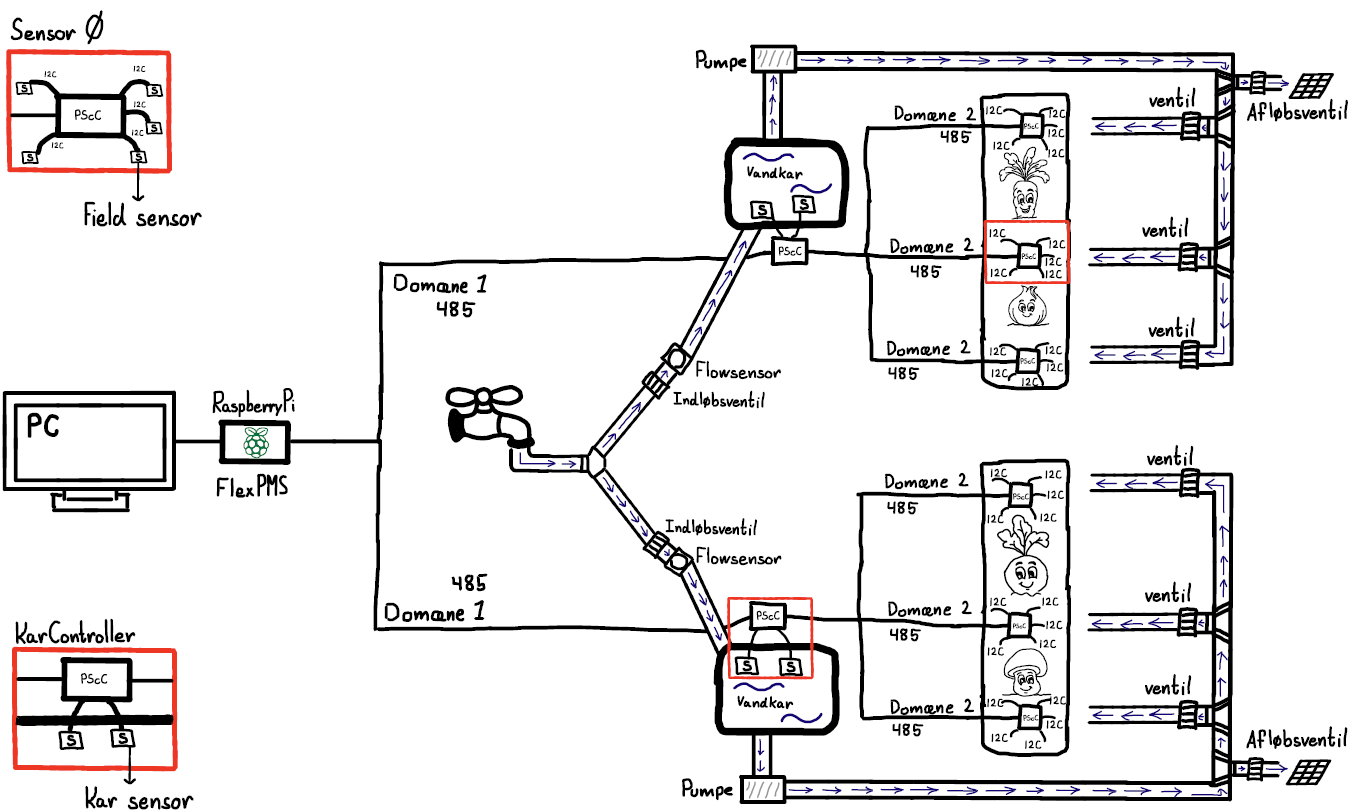
\includegraphics[width=\textwidth]{SystemArkitektur/AVS}
    \caption{Grafisk systembeskrivelse}
    \label{fig:graf_sys}
\end{figure}
Figur \ref{fig:graf_sys}, er en grafisk systembeskrivelse af det overordnede system som har indholder følgende:
\begin{itemize}
\item De blå pile illustrer vandvejen gennem vandslanger i forhold til kar, ventiler og pumpen. 
\item Ud fra var vandkaret sider en PSoC, som er forbundet til sensorerne på karet og de PSoC's der ligger i gromediet/plantekasserne.
\item I plantekasserne ligger der nogle PSoC's som bliver kaldt for \glslink{sensoroe}{Sensor Øer}, disse er forbundet til nogle sensorer der tager nogle forskellige målinger. 
\end{itemize}
\section{System diagrammer}

%!TEX root = ../../main.tex

\subsection{System Domænemodel}

\systemDomainModel{0.82}{System}{AVS}

\subsection{System BDD}

\systemBDD{0.82}{System}{AVS}

\subsubsection{CentralControl}
CentralControl er systemets centrale computer. Det er gennem dette delsystem, at brugerens interaktion bliver behandlet og formidlet videre til andre delsystemer. CentralControl driver en webserver med dertilhørende web-applikation (GUI), som tillader brugeren at interagere med systemet gennem sin web-browser. Webserveren kommunikerer med et stykke centralt software, FlexPMS.

\subsubsection{GUI}
GUI er den brugergrænseflade, som brugeren kan tilgå systemet gennem.

\subsubsection{FlexPMS}
FlexPMS (Flexible Plant Management System) softwaren er bindeleddet mellem GUI og de andre delsystemer. FlexPMS afvikles konstant på CentralControl, og håndterer at sende kommandoer til og opsamle data fra KarControl. FlexPMS kommunikerer med de andre delsystemer gennem enhedsdrivers, som er udviklet til – og installeret på – CentralControl.

\subsubsection{Database}
Databasen gemmer alle indstiller lavet af brugeren gennem GUI.

\subsubsection{KarControl}
KarControl er en styring, som formidler og håndterer al datakommunikation og kommandoer relateret til ét kar. KarControl formidler kommandoer sendt fra CentralControl videre til hardware koblet på det pågældende kar (f.eks. at åbne og lukke for ventiler), samt formidler måledata fra sensorer tilbage til CentralControl. KarControl ved hvilken pH-værdi karret skal have, samt hvilken koncentration af gødning og jordfugtighed planterne, der er tilkoblet karret, skal have. KarControl sørger selv for, at vedligeholde disse værdier. CentralControl giver KarControl besked, når der foretages ændringer af disse værdier.

\subsubsection{Sensor Ø}
Sensor Ø’er giver mulighed for at måle (f.eks. jordfugtighed) over et større areal ved, at Sensor Ø’erne spredes over området, hvor planterne gror, og har hver især tilsluttet sensorer. Dermed kan man måle jordfugtighed lokalt for området omkring Sensor Ø’en og styre vandtilførslen specifikt for planterne, som står i området.

\subsubsection{RSConverter}
RSConverter konverterer fra RS485 til RS232 når der modtages data, og fra RS232 til RS485 når der afsendes data.


\subsection{System Allokeringsdiagram}

\systemAllokeringsDiagram{0.82}{System}{AVS}









\newpage
\section{CentralControl diagrammer}
\subsection{CentralControl IBD}

\systemIBD{0.82}{CentralControl}{CentralControl}

\subsection{Signal beskrivelser}

\begin{table}[H]
\centering
{\rowcolors{2}{white!80!black!30}{white!70!black!60} %farver på hver anden række -starter på 3
\setlength{\arrayrulewidth}{0.2mm}					 %tykkelse på linier 
\setlength{\tabcolsep}{10pt}						 %indryk i celle 
\renewcommand{\arraystretch}{1.5}					 %højden på tabelrum
\center
\begin{tabular}{|p{20mm}|p{40mm}|p{30mm}|p{30mm}|}		 %længden på alle rum
\hline

\multicolumn{4}{|>{\columncolor{white!20!black!90}}m{14.20cm}|}{\textcolor{white}{\large{\textbf{Signal beskrivelser}}}} \\\hline
\rowcolor{white!70!black!60}
\textcolor{black}{\large{\textbf{Navn}}}&
\textcolor{black}{\large{\textbf{Definition}}}&	
\textcolor{black}{\large{\textbf{Område}}}&
\textcolor{black}{\large{\textbf{Kommentar}}}\\
\hline
KarBus				& RS485 bus til kommunikation mellem enheder &	 	& Differentielt bussystem  \\
Data485				& RS485 bus til kommunikation mellem enheder &	 	& internt signal   \\
Data232				& RS485 konverteret til logisk niveau		 &	 	& Signal efter konvertering  \\
PMSConn				& Database forbindelse						 &		& Til at skrive log \\
GUIConn				& Database forbindelse						 &		& Til at hente og skrive indstillinger samt log \\
ControlConn			& Socket forbindelse fra GUI til FlexPMS	 &		& Til at sende kommandoer fra GUI til FlexPMS \\
html				& Http protokol								 &		& Fobindelse til brugerens browser \\
\hline
\end{tabular}
}
\caption{signal beskrivelser for CentralControl}
\label{table:SignalBeskrivelserKarControl}
\end{table}


\newpage
\section{KarControl diagrammer}
%!TEX root = ../../main.tex

\subsection{KarControl BDD}
\systemBDD{0.82}{KarControl}

\subsubsection{KarGruppe}
KarGruppe er den overordnede betegnelse for et vandkar med tilførende pH-værdi og gødningskoncentration. KarGruppen består af diverse sensorer og aktuatorer, og styrer et vilkårligt antal Sensor Ø’er. KarGruppen er styret af en controller, KarControl.

\subsubsection{Indløbsventil}
Indløbsventilen åbner og lukker for vandtilføjelsen til karret. Den bruges i forbindelse med, at der skal fyldes vand på karret. Det antages, at indløbsventilen er tilsluttet en vandforsyning, som altid er åben.

\subsubsection{Afløbsventil}
Afløbsventilen åbner og lukker for, at vand kan løbe ud af karret. Den bruges i forbindelse med, at karret skal tømmes.

\subsubsection{pH-Sensor}
pH-sensoren målet pH-værdien af gødningsblandingen i karret.

\subsubsection{Vandpumpe}
Vandpumpen pumper vand fra karret ud til Sensor Ø’erne.

\subsubsection{Flowmåler}
Flowmåleren måler mængden af vand, som tilføres karret gennem Indløbsventilen.

\subsection{KarControl IBD}
\systemIBD{0.82}{KarControl}{KarControl}

\subsubsection{RSIn}
RSConverter konverterer mellem RS485 og UART 232 når der skal kommunikeres med CentralControl.

\subsubsection{RSOut}
RSConverter konverterer mellem RS485 og UART 232 når der skal kommunikeres med Sensor Ø'er.

%\subsection{KarControl Allokeringsdiagram}
%\systemAllokeringsDiagram{0.82}{KarControl}{KarControl}

\subsection{Signalbeskrivelser KarControl}
\systemSignaler{KarControl} {
KarBus				& RS485 bus til kommunikation mellem enheder & Binary 1 (OFF)
																   (Voa-Vob<-200 mV)
																   Binary 0 (ON)
																  (Voa-Vob>+200 mV)	 	& Differentielt bussystem \\
OeBus				& RS485 bus til kommunikation mellem enheder & Binary 1 (OFF)
																   (Voa-Vob<-200 mV)
																   Binary 0 (ON)
																  (Voa-Vob>+200 mV)	 	& Differentielt bussystem \\
Data485				& RS485 bus til kommunikation mellem enheder & Intern:SW-signal		& Internt signal fra RSconverter til KarGruppe \\
Data232				& RS485 konverteret til logisk niveau		 & Intern:SW-signal 	& Konverteret signal fra RSconverter til Controller  \\
EnableIndløb		& Signal til at lukke vand ind i kar		 & Logisk:0-5V			& Signal til styring af Indløbsventil   \\
EnableAfløb			& Signal til at lukke vand ud af kar		 & Logisk:0-5V			& Signal til styring af Afløbsventil   \\
EnableVandpumpe		& Styre signal til pumpe			   	     & Logisk:PWM 0-5V 		& Signal til PWM-styring af Vandpumpe	\\
Puls				& Takttæller af flow				   	 	 & Logisk:0-5V 			& Retursignal fra flowtæller \\
pH					& Analog signal fra pH måler			 	 & Analog:-420mV-420mV  & Analogt sensorsignal \\
Indløb				& vandstyring i kar							 & Vandflow   			& Vandtilførsel til karret \\
Afløb				& vandstyring i kar	 						 & Vandflow  			& Vandtilafledning fra karret \\
Dossering			& vandstyring til planter					 & Vandflow    			& Vandtilførsel til dosering \\
}

\newpage
\section{Sensor Ø diagrammer}
%!TEX root = ../../main.tex

\subsection{Sensor Ø BDD}
\systemBDD[Sensor_oe]{0.82}{Sensor Ø}

\subsubsection*{Sensor Ø Control}
Sensor Ø Control tager imod kommandoer fra KarControl, som instruerer omkring åbning og lukning af Doseringsventil. KarControl anmoder også om, at Sensor Ø Control skal sende måledata fra sensors, som er tilkoblet Sensor Ø’en.

\subsubsection{Doseringsventil}
Doseringsventilen åbner og lukker for vandtilførslen til planterne i området omkring Sensor Ø’en, som Doseringsventilen er tilkoblet. Når KarControl tænder for Vandpumpen kan de enkelte Sensor Ø’ers Doseringsventiler være åbne eller lukkede alt efter, om planterne omkring Sensor Ø’en har brug for vand.

\subsubsection{Fieldsensor}
Fieldsensor er en generalisering af alle slags sensorer, som kan tilsluttes Sensor Ø’en. Vilkårligt mange sensorer kan tilkobles en bus, og kommunikere med Sensor Ø Control gennem en standardiseret protokol. Sensor kan kun aflevere målinger når de bliver bedt om at levere dem.

\subsection{Sensor Ø IBD}
\systemIBD{0.82}{Sensor_oe}{Sensor Ø}

%\subsection{Sensor Ø Allokeringsdiagram}
%\systemAllokeringsDiagram{0.82}{Sensor_oe}{Sensor Ø}

\subsection{Signal beskrivelser}
\systemSignaler[SensorOe]{Sensor Ø}{
oeData				& Buskommunikation efter konvertering fra 485 &	 	& UART kommunikation fra 485 bussen  \\
oeBus				& RS485 bus til kommunikation mellem enheder  &	 	& Differentielt bussystem  \\
sensorData			& Signal på I2C bus							  &	 	& Kan være flere forskellige signaler alt efter sensor type   \\
ventilCtrl			& Signal til styring af doserings ventil	  &	0-5V& Bruges til at styre mængden af vand til planterne \\
vand				& Dette er flow'et af vand 					  &		& \\
}

\newpage
\section{Fieldsensor diagrammer}
%!TEX root = ../../main.tex

\subsection{Fieldsensor BDD}
Dette er vores modelLibrary af de sensorer der matcher Fieldsensor specifikationerne

\systemBDD{0.7}{Fieldsensor}

\subsection{Signalbeskrivelser Fieldsenser}
\systemSignaler{Fieldsensor}{
sensorData				&  I2C kommunikation			& Logisk: 0-5V 	&  Kommunikation fra sensorer til Fieldsensor\\
}

\newpage
\section{Jordfugt sensor diagrammer}
%!TEX root = ../../main.tex

Jordfugt sensoren måler en strøm igennem jorden. Denne strøm vil variere med hensyn til fugtigheden som derfor vil resultere i en spændingsændring på indgangen af analog til digital converteren. Denne spænding bruges til at udregne fugtigheden i procent

\subsection{Jordfugt sensor BDD}
\systemBDD[Sensor_Jordfugt]{0.83}{Jordfugt sensor}

\subsection{Jordfugt sensor IBD}
\systemIBD{0.83}{Sensor_Jordfugt}{Jordfugt sensor}

\subsection{Signal beskrivelser}
\systemSignaler{Jordfugt sensor}{
				&  			&	 	&   \\
				&  			&	 	&   \\
}

\newpage
\section{pH-sensor diagrammer}
%!TEX root = ../../main.tex

\newpage
\section{Ventilstyring diagrammer}
%!TEX root = ../../main.tex
\section{Ventilstyring}
Til styring af indløb til / afløb fra vandkaret anvendes 2 Hydraelectric Magnetventiler med tilhørende MOSFET-styringskredse. En magnetventil virker ved at det interne relæ bliver aktiveret når der påtrykkes en DC-spænding, evt. i form af et PWM-signal, hvor ved gennemstrømningen kan reguleres, når dette sker åbnes der for gennemgang i ventilen. I det interne relæ sidder en spole, og spolens viklinger medfører en ohmsk modstand. Når der påtrykkes en spænding skabes et magnetfelt omkring spolen, dette felt holder ventilen åben. Når ventilen ønskes lukket, afbrydes spændingen. Dette skaber en problematik hvor strømmen igennem spolen ikke kan ændre sig på samme hurtige måde aom spændingen. Da den fysiske forbindelse til spolen er afbrudt vil spolen selv inducere en modsatrettet spænding for at komme af med strømmen. Dette er et problem da så høje spændinger potentielt er skadeligt for tilkoblede komponenter, men som løsning implementeres en ”flyback diode” parallelt med spolen i reverse bias-konfiguration, derved har strømmen en løbebane, og spolen forhindres i at inducere den høje spænding. Den implementerede kontrolkreds ses på figur \ref{screenshot:ventilStyringskreds} på side \pageref{screenshot:ventilStyringskreds}.
I databladet er oplyst at ventilen benytter 12V, afgiver 6W, dette giver et beregnet strømforbrug på 500mA, se beregning herunder:

\begin{figure}[!h]
		\begin{align*}
			P &= 6 VA \\ 
			V &= 12 V \\
			I &= \frac{P}{V} \eqref{1}\\ 
			&= 500mA
		\end{align*}
\label{eq:ventilA}
\caption{Beregning af strømforbrug i magnetventil}
\end{figure}

Derudover er den interne modstand beregnet til: 

\begin{figure}[!h]
	\begin{align*}
		V &= 12 V \\ 
		I &= 500 mA \\
		R &= \frac{V}{I} \\ 
		&= 24 \Omega
	\end{align*}
\caption{Beregning af indre modstand}
\label{eq:ventilOhm}
\end{figure}

Styringskredsen skal på baggrund af dette designes til at håndtere en strøm på 500mA, og en spænding på 12V. 


\newpage
\subsection{MOSFET-styringskreds}
Til styringslkredsen er valgt at benytte en N-channel IRLZ44Z-MOSFET transistor i common-source-konfiguration. Denne type transistor er logic-level kompatibel, og har spænding/strøm-grænseværdier der opfylder ovenstående krav.  
Logic-level kompatible betyder at $ V_{GS(th)} < 5V $ og derved kan MOSFET`en, alene drives fra en MCU, her en PSoC.
$ V_{GS(th)} $ er den threshold-spænding hvor transistoren går ”on”.


Det ses af grafen på figur \ref{screenshot:GateToSourceVoltage}, at MOSFET`en ved en $ V_{GS} = 5V $, (ved $T_J = 25)$ tillader en strøm på 100A, dette er mere end rigeligt til opgaven.

\begin{figure}[!h]
	\centering
	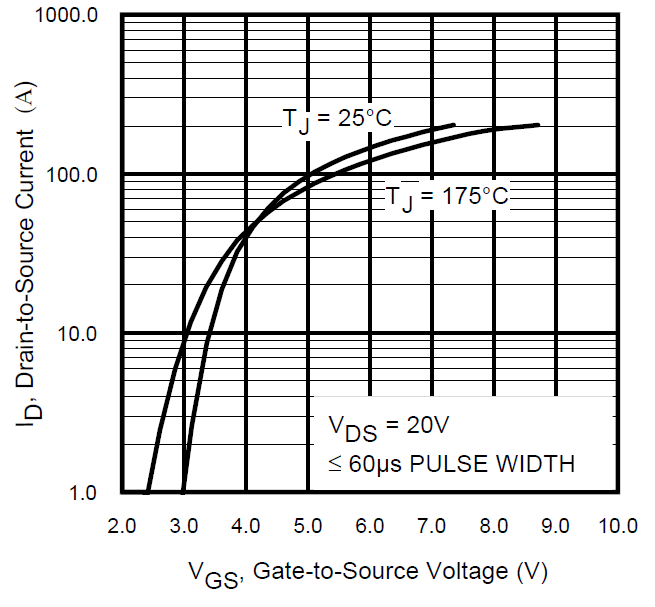
\includegraphics[scale=0.3]{../Hardware/Ventilstyring/Screenshots/DatasheetGateSourceVoltage}
	\caption{Datablad: Gate to Source voltage, fra databladets (Fig. 3, s.3)}
	\label{screenshot:GateToSourceVoltage}
\end{figure}

Ydermere kan det være interessant at se på hvor varm transistoren bliver under operation. Herved kan det udledes om der behøves ekstern køling eks. i form af en heat-sink.
Følgende værdier hentet fra databladet: 

\begin{figure}[!h]
	\begin{center}
		\begin{tabular}{ l l }
 			Drain to Source modstand:          & $R_{DS}=11 m\Omega$ \\ 
 			Strøm der trækkes af af relæet:    & $I = 500 mA$ \\  
 			Junction-to-Ambient modstand:      & $R_{\theta JA}=62 C/W$ \\   
 			Max junction temp:                 & $Temp_{jun}=175 C$ \\
 			Ambient temp:                      & $Temp_{amb}=25 C$ \\
		\end{tabular}
	\end{center}
\caption{Værdier hentet fra datablad}
\end{figure}

Til beregningen benyttes formlen for afsat effekt: 

\begin{figure}[!h]
		\begin{align*}
		P_{afsat} &= R_{DS}*I^2 \\ 
		&= 2.75 mW
		\end{align*}
\caption{Afsat effekt i MOSFET}
\label{eq:afsatEffektMOSFET}
\end{figure}

Her ses det at under operation af ventilen afgiver transistoren 2,75 mW i varme. Ydermere noteres det, at den maksimale effekt der kan afsættes uden at der behøves heat-sink er beregnet til 447.561mW. 

\begin{figure}[!h]
	\begin{align*}
		Temp_{max} &= \frac{(Temp_{jun}-Temp_{amb})}{R_{\theta JA}} \\ 
		&= 447.561 mW
	\end{align*}
\caption{Max Temperatur uden heat-sink}
\label{eq:maxMOSFETeffekt}
\end{figure}

Da der kun afsættes 2,75mW ved operation, er der ingen grund til at implementerer en heat-sink.


\subsubsection{Design af styringskredsløb}
På figur \ref{screenshot:ventilStyringskreds}, ses MOSFET-styringskredsløb, PSoC`ens ”0” og ”1” er her simuleret ved en frekvensgenerator med tilpas lav frekvens.

\begin{figure}[!h]
	\centering
	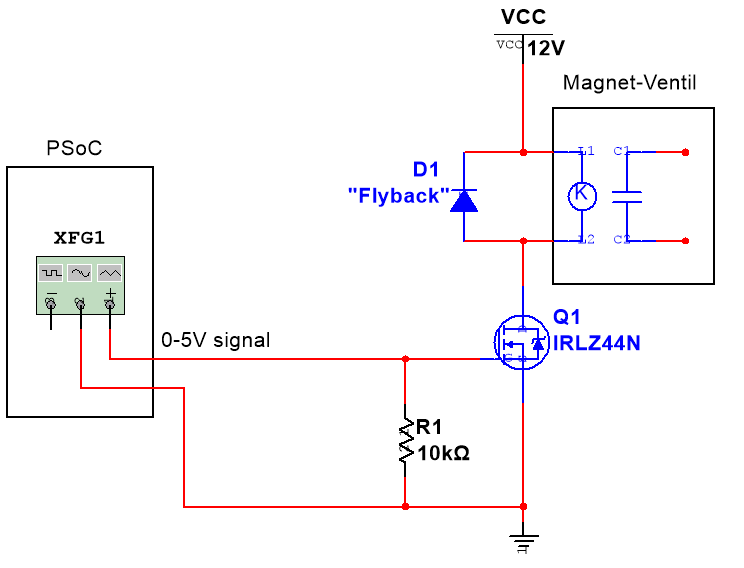
\includegraphics[height=6cm]{../Hardware/Ventilstyring/Screenshots/VentilStyringskreds}
	\caption{Styringskredsløb til magnetventil}
	\label{screenshot:ventilStyringskreds}
\end{figure}

\paragraph{MOSFET-transistoren} \hspace{0pt} \\
Transistoren implementeres i common-source-konfiguration, for at et positivt signal på GATE ”åbner” transistoren, og da den er en logic level
model, stammer signalet direkte fra PSoCen. 

\paragraph{Ground-modstanden} \hspace{0pt} \\
Der implementeres en modstand $R_1$ fra Gate til GND for at transistoren forbliver lukket (Gate trækkes til GND) hvis indgangssignalet til Gate afbrydes, dermed undgås det at GATE-signalet ”flyver” og transistoren potentielt kan stå og switche on/off hvis GATE afbrydes. $R_1$ implementeres med en $10k\Omega$s modstand, og virker som en standard ”pull down” resistor.

\paragraph{Flyback-diode} \hspace{0pt} \\
Derudover implementere der, som førnævnt en ”flyback” diode, for at give strømmen en løbebane når relæet afbrydes. På denne måde indgås den høje $V_{peak}$ som spolen eller ville inducere, når der lukkes af for strømmen ændres monumentalt. Typen af diode, vælges ud fra følgende parametre:


\begin{description}
 \item[•] Hvilken strøm vil løbe i dioden
 \item[•] Hvilken Peak-spænding vil være over dioden
\end{description}

\subparagraph{Diode-strøm} \hspace{0pt} \\
Strømmen der vil løbe i dioden er givet fra databladet til  3A, derved skal den valgte diode kunne klare at lede max 3A, dette sker i forhold til spolens tidskonstant, $\tau$, hvor efter strømmen vil falde i løbet af $ 5 \tau$.

\subparagraph{Peak-spænding} \hspace{0pt} \\
Peak-spændingen fra spolen er realiseret i laboratoriet til 60V. 

På baggrund af disse 2 værdier, vælges 1N4007, denne diode er, ifølge databladet i stand til at klare 1kVp, og 30A. Dette er tilstrækkeligt i denne situation.


\newpage
\section{Vandpumpestyring diagrammer}
%!TEX root = ../../main.tex

Vi bruger en vandpumpe på alle vores kar.

\subsection{Vandpumpestyring BDD}
Her under ses et diagram over den generalle opbygning af vandpumpe styringen denne gør sig gældende for alle vandpumper i systemet

\systemBDD{0.5}{Vandpumpestyring}

\subsection{Vandpumpestyring IBD}
Her ses så de interne forbindelser i Vandpumpestyringen 

\systemIBD{0.5}{Vandpumpestyring}{Vandpumpestyring}

\subsection{Signal beskrivelser}
\systemSignaler{Vandpumpestyring}{
cV				& Pwm signal til Mosfet kredsløbet 			&	0-5V 		&  Bestemmer om Vandpumpen roterer \\
vand			& Vand der flyder gennem Vandpumpen			& 0 - 17l/min	& Bestemmer mængden af vand til dosering	\\
}

\newpage
\section{Teknologiundersøgelser}
%!TEX root = ../../main.tex
%!TEX root = ../../../main.tex
\subsection{RS485}
Kommunikationen som foregår i systemet imellem brugerinterfacet (Devkit 8000), KarControl (PSoC 4) og de enkelte forgreninger (PSoC 4) skal kunne kommunikere over længere afstande. De allerede kendte busser, SPI og I2C, har begge en maksimal rækkevidde på 1,5m. Vi har derfor været nødsaget til at finde et bedre alternativ. Problemet over længere afstande kan være:

\begin{itemize}
\item Kapacitet i ledningerne
\item Støj fra omkringliggende elektronik
\end{itemize}

For at løse disse problemer, har vi undersøgt RS485-kommunikation. RS485 er en standard som definerer de elektriske karakteristika af sendere og modtagere på en differentiel bus. Ved 2 ledninger kan man opnå half-duplex, og ved 4 ledninger kan man opnå full duplex. Ledningerne i bussen skal være parsnoede. Ved afstande helt op til 1200m, er det muligt at køre med hastigheder på op til 100kbit/s. RS485 er en udbygning af RS422, hvor man har muligheden for at vælge hvorvidt det er input- eller output-driverne som er aktive. Den fysiske konfiguration af bussen skal forbindes som én linje.
Dvs. at man kan f.eks. ikke parallel-forbinde 5 enheder direkte til en master, de skal derimod serieforbindes. Bussen termineres i begge ender, med en modstand som svarer til kablernes egen modstand, normalt 120ohm for parsnoede kabler, imellem de 2 bus-forbindelser.
\\\\
Man vil gerne opnå at masteren er centreret i bussen, og at termineringsmodstandene derved er på 2 slaver. Ved at gøre dette, vil afstanden fra masteren til slaverne være så lille som mulig, og derved vil signal-styrken være bedst.
\\\\
RS485 er KUN en elektrisk definition af bussen, og ikke en kommunikationsprotokol. Dette giver mulighed for at skrive sin egen protokol. Standarden anbefaler dog, at man bruger kommunikationsprotokollen TSB-89.


\fixme{der skal indsættes resten af teknologi undersøgelserne}



\newpage
\section{Overordnede Sekvensdiagrammer}
%!TEX root = ../../main.tex

Her vises overordnede sekvensdiagrammer for hver use case, til at give et overblik over systemets funktionalitet, så det gerne skulle blive lettere at forstå systemmet, og dets interaktion med aktører. Dette skulle gerne vise et bedre indblik på de forskellige interaktioner for den ydre verden. 

\subsection{Overordnede sekvensdiagram for use case 1 - aflæse målinger}
Diagrammet viser interaktion mellem system og bruger for use case 1 - aflæse målinger.

\begin{figure}[H]
    \centering
    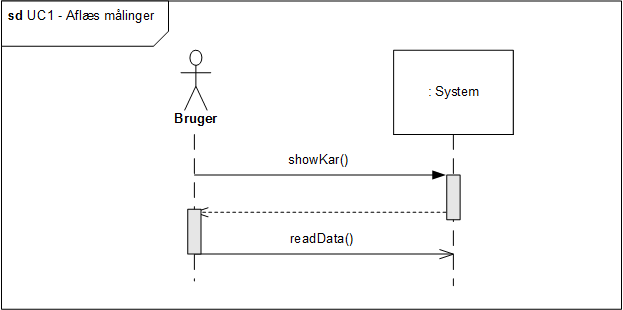
\includegraphics[width=0.8\textwidth]{Systemarkitektur/OverordnedeSekvensdiagrammer/sd_UC1.PNG}
    \caption{sd - use case 1}
    \label{fig:sd_UC1}
\end{figure}

\subsection{Overordnede sekvensdiagram for use case 2 - manuel vanding}
Diagrammer viser interaktion mellem system og bruger for use case 2 - manuel vanding.

\begin{figure}[H]
    \centering
    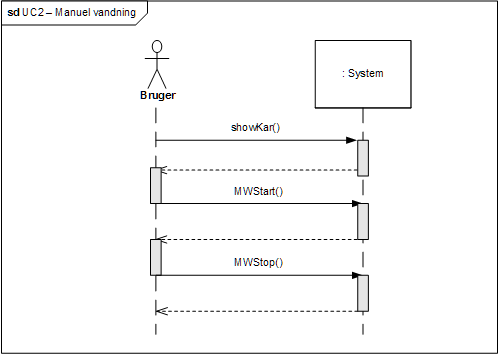
\includegraphics[width=0.8\textwidth]{Systemarkitektur/OverordnedeSekvensdiagrammer/sd_UC2.PNG}
    \caption{sd - use case 2}
    \label{fig:sd_UC2}
\end{figure}


\subsection{Overordnede sekvensdiagram for use case 3 - Indtast pH-værdien}
Diagrammer viser interaktion mellem system og bruger for use case 3 - Indtast pH-værdien.

\begin{figure}[H]
    \centering
    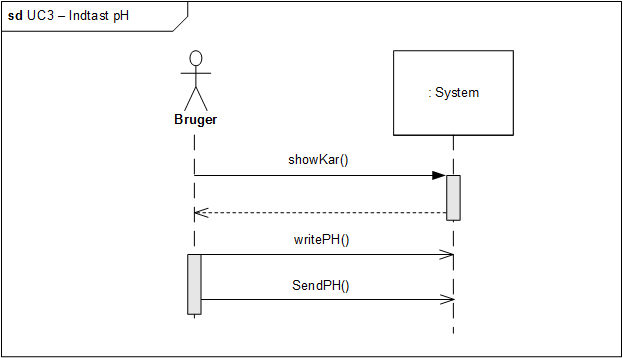
\includegraphics[width=0.8\textwidth]{Systemarkitektur/OverordnedeSekvensdiagrammer/sd_UC3.PNG}
    \caption{sd - use case 3}
    \label{fig:sd_UC3}
\end{figure}

\subsection{Overordnede sekvensdiagram for use case 4 - Indtast pH-værdien}
Diagrammer viser interaktion mellem system og bruger for use case 4 - Indtast volumen.

\begin{figure}[H]
    \centering
    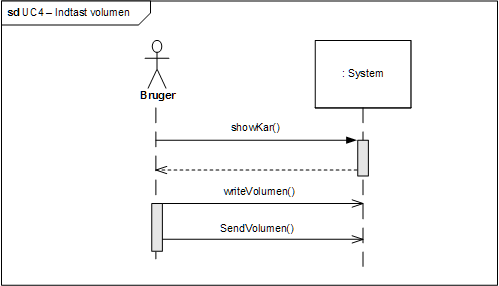
\includegraphics[width=0.8\textwidth]{Systemarkitektur/OverordnedeSekvensdiagrammer/sd_UC4.PNG}
    \caption{sd - use case 4}
    \label{fig:sd_UC4}
\end{figure}

\subsection{Overordnede sekvensdiagram for use case 5 - Indtast pH-værdien}
Diagrammer viser interaktion mellem system og bruger for use case 5 - Opret kar.

\begin{figure}[H]
    \centering
    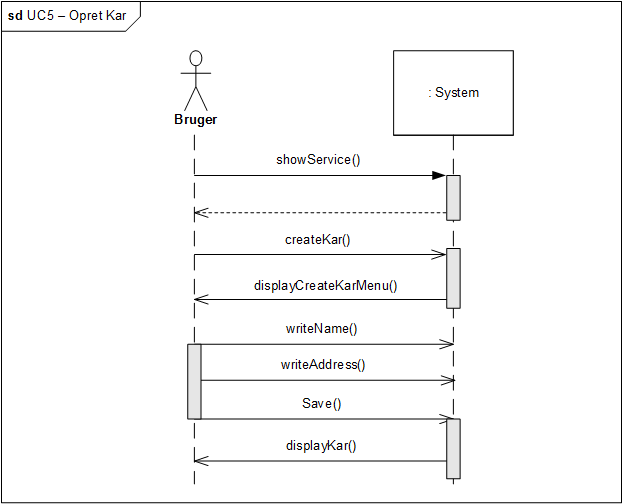
\includegraphics[width=0.8\textwidth]{Systemarkitektur/OverordnedeSekvensdiagrammer/sd_UC5.PNG}
    \caption{sd - use case 5}
    \label{fig:sd_UC5}
\end{figure}

\subsection{Overordnede sekvensdiagram for use case 6 - Indtast pH-værdien}
Diagrammer viser interaktion mellem system og bruger for use case 6 - Slet kar.

\begin{figure}[H]
    \centering
    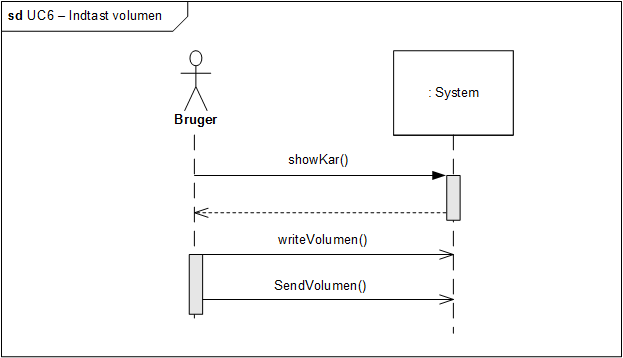
\includegraphics[width=0.8\textwidth]{Systemarkitektur/OverordnedeSekvensdiagrammer/sd_UC6.PNG}
    \caption{sd - use case 6}
    \label{fig:sd_UC6}
\end{figure}

\newpage
\section{Klasseidentifikation}
%!TEX root = ../../main.tex

I system domænemodellen, som ses på figur \ref{fig:System_Domain_Model}, kan det ses at der blev identificeret nogle konceptuelle klasser, hvor hver klasse har til ansvar at løse et specifikt problem. Ud fra dette vil vi gerne se på hvilke domæner og grænseflader der er. Hvor grænsefladerne er det der skal anvendes når dele af systemmet skal kommunikerer og domæne står for de resterende problemer. Så ud fra domænemodellen er følgende grænseflade- og domæneproblemer defineret:
\begin{itemize}
	\item Grænseflader:
		\begin{itemize}
			\item Bruger Grænseflade
			\item GUI grænseflader
			\item FlexPMS grænseflader 
			\item Kar grænseflader
			\item SensorØ grænseflader
		\end{itemize}
	\item Domæne:
	\begin{itemize}
			\item Håndtering af de forskellige setværdier (pH, volumen, jordfugtighed osv.)
			\item Håndtering af målinger
			\item Håndtering af Kar data 
			\item Håndtering af SensorØ data 
		\end{itemize}
\end{itemize} 

Ud fra dette udarbejdes applikationsmodeller. Hver applikationsmodel har til opgave at vise de klasser som er involveret i de forskellige use cases. Dette håndteres af kontrolklassen. grænseflade- og domæneklasserne er bestem ud fra det overstående så der er identificeret følgende klasser:

\begin{itemize}
	\item Boundaryklasser:
		\begin{itemize}
			\item \textbf{GUI} - Brugergrænseflade mellem bruger og system
			\item \textbf{Database} - Grænseflade mellem GUI og FlexPMS
			\item \textbf{Protokol} - Bussystemerne der kommunikere med vores hardware 
		\end{itemize}
	\item Domainklasser:
	\begin{itemize}
			\item \textbf{Sensor} - Måler de forskellige data (pH, volumen, jordfugtighed osv.)
			\item \textbf{Kar} - Håndterer de specifikke data for de individuelle kar
			\item \textbf{SensorØ} - Håndterer de specifikke data for de individuelle SensorØ'er
	\end{itemize} 
\end{itemize} 
 
Ud fra use casene og de definerede klasser, kan der nu oprettes applikationsmodeller. Applikationsmodellerne
består af henholdsvis en kontrolklasse der varetager use casens forløb, samt de definerede domain-
og boundaryklasser, som kontrolklassen skal bruge for at opfylde dette. Da der er mange af use casene der ligner hinanden er nogle af dem slået sammen i en applikationsmodel. 


\subsection{Klassediagram for use case 1 - Aflæs data}

\begin{figure}[H]
    \centering
    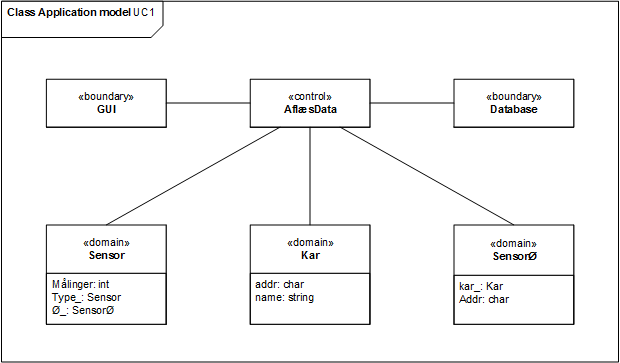
\includegraphics[width=0.8\textwidth]{Systemarkitektur/KlasseDiagrammer/1_AflaesData.PNG}
    \caption{Applikationsmodel for UC1}
    \label{fig:app_uc1}
\end{figure}

Dette klassediagram er benyttet til at identificere nødvendige klasser for at udføre use case 1.
Nedenfor er beskrives kort klassernes ansvar for use case 1.
\\\\
\textbf{AflæsData:}\\
varetager og koordinerer interaktionen mellem de interne klasser i henhold til use casen.
\\\\
\textbf{GUI:}\\
Grænseflade mellem, system go bruger, hvor brugeren aflæser de målte data. 
\\\\

\subsection{Klassediagram for use case 2 - Manuel vanding}
\begin{figure}[H]
    \centering
    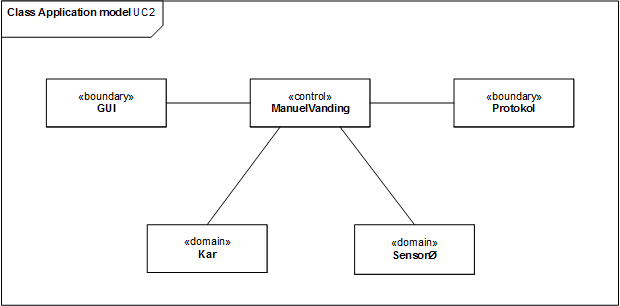
\includegraphics[width=0.8\textwidth]{Systemarkitektur/KlasseDiagrammer/2_ManuelVanding.PNG}
    \caption{Applikationsmodel for UC2}
    \label{fig:app_uc2}
\end{figure}

Dette klassediagram er benyttet til at identificere nødvendige klasser for at udføre use case 2.
Nedenfor er beskrives kort klassernes ansvar for use case 2.
\\\\
\textbf{Manuel vanding:}\\
varetager og koordinerer interaktionen mellem de interne klasser i henhold til use casen.
\\\\
\textbf{GUI:}\\
Grænseflade mellem, system go bruger, hvor brugeren kan aktivere den manuelle vanding. 
\\\\
\textbf{Protokol:}\\
Bussystem, der kommunikerer med vores hardware, så manuel vanding kan aktiveres.
\\\\

\subsection{Klassediagram for use case 3 og 4 - Indtast data}

\begin{figure}[H]
    \centering
    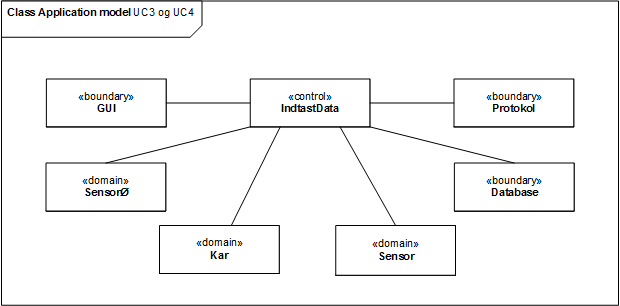
\includegraphics[width=0.8\textwidth]{Systemarkitektur/KlasseDiagrammer/3+4_IndtastData.PNG}
    \caption{Applikationsmodel for UC3 og UC4}
    \label{fig:app_uc2}
\end{figure}

Dette klassediagram er benyttet til at identificere nødvendige klasser for at udføre use case 3 og 4.
Nedenfor er beskrives kort klassernes ansvar for use case 3 og 4.
\\\\
\textbf{IndtastData:}\\
varetager og koordinerer interaktionen mellem de interne klasser i henhold til use casen.

\textbf{GUI:}\\
Grænseflade mellem, system go bruger, hvor brugeren Indtaste de ønskede data. 
\\\\

\textbf{Database:}\\
Grænseflade mellem GUI og FlexPMS, hvor de  indtastede data bliver gemt. 
\\\\

\subsection{Klassediagram for use case 5 og 6 - Kar manipulation}

\begin{figure}[H]
    \centering
    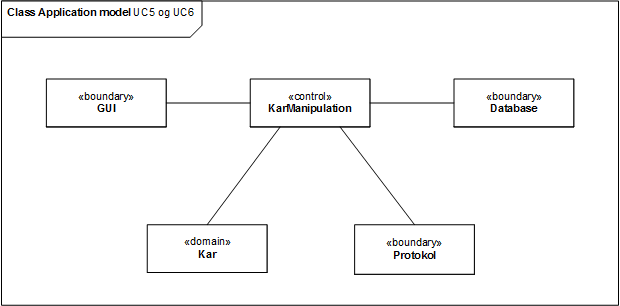
\includegraphics[width=0.8\textwidth]{Systemarkitektur/KlasseDiagrammer/5+6_KarManipulate.PNG}
    \caption{Applikationsmodel for UC5 og UC6}
    \label{fig:app_uc2}
\end{figure}

Dette klassediagram er benyttet til at identificere nødvendige klasser for at udføre use case 5 og 6.
Nedenfor er beskrives kort klassernes ansvar for use case 5 og 6.
\\\\
\textbf{KarManipulation:}\\
Varetager og koordinerer interaktionen mellem de interne klasser i henhold til use casen.
\\\\
\textbf{GUI:}\\
Grænseflade mellem, system go bruger, hvor brugeren kan oprette og slette kar. 
\\\\

\textbf{Database:}\\
Grænseflade mellem GUI og FlexPMS, hvor det forskellige kar bliver gemt med deres data. 
\\\\

\newpage
\section{Grænsefladebeksrivelser}
%!TEX root = ../../main.tex

\subsection{Ventilstyring Grænsefladebeskrivelse}

Ventilstyring er en grænseflade til systemet, modulet omsætter digital styring fra PSoC'en til analog aktuation i mangetventilen der kontrollerer vandtilførsel, udledning, samt dosering ved karret. 
Modulet tager, som input, et digitalt signal 0-5V. Dette omsættes til analog styring af ventilen. 
Derudover tilføres kontrolkredsen 12V som forsyningsspænding. fig.\ref{screenshot:tabel1},s.\pageref{screenshot:tabel1}

\begin{figure}[H]
	\centering
	\includegraphics[scale=0.6]{../Projektdokumentation/Systemarkitektur/Graenseflader/Screenshots/tabel1}
	\caption{Grænsefladebeskrivelse: Ventilstyring}
	\label{screenshot:tabel1}
\end{figure}


\subsection{Doseringspumpe Grænsefladebeskrivelse}

Doseringspumpen er ligeledes en grænseflade til systemet, modulet omsætter et digital PWM-signal fra PSoC'en til en procentvis styring af doseringspumpen så den kan kører i flere etaper. Modulet tager, som input, et digitalt PWM-signal 0-5V. Dette omsættes til analog styring i doseringspumpen. 
Derudover tilføres kontrolkredsen 12V som forsyningsspænding. fig.\ref{screenshot:tabel2},s.\pageref{screenshot:tabel2}  

\begin{figure}[H]
	\centering
	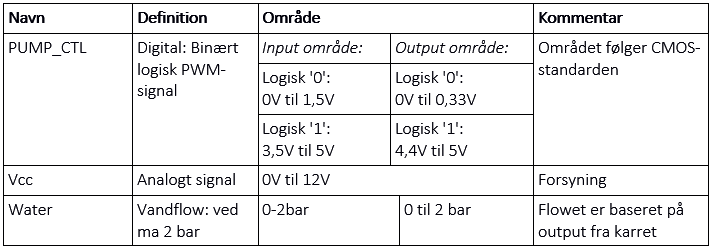
\includegraphics[scale=0.6]{../Projektdokumentation/Systemarkitektur/Graenseflader/Screenshots/tabel2_Pumpe}
	\caption{Grænsefladebeskrivelse: Doseringspumpe}
	\label{screenshot:tabel2}
\end{figure}


\subsection{Flowsensor Grænsefladebeskrivelse}
Flowsensor fungerer som grænseflade til systemet, modulet omsætter vandflow i sensoren til et digital PWM-signal der angiver hvor meget vand der flyder igennem sensoren. Modulet forsynes med +5V forsyning, samt GND, og afgiver PWM-signal 
Dette PWM omsættes via et eksternt counterkredsløb til at give logisk '1' ved hver 10. count. Dette trækker et interrupt i PSoC'programmet.fig.\ref{screenshot:tabel3},s.\pageref{screenshot:tabel3}

\begin{figure}[H]
	\centering
	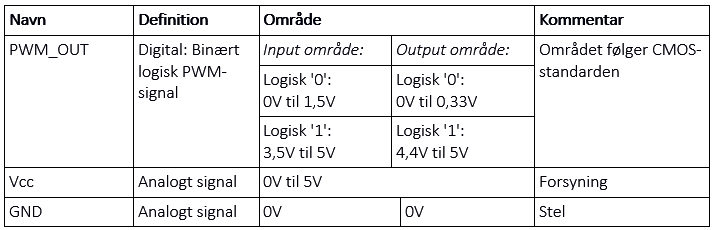
\includegraphics[scale=0.6]{../Projektdokumentation/Systemarkitektur/Graenseflader/Screenshots/tabel3_Flowsensor}
	\caption{Grænsefladebeskrivelse: Flowsensor}
	\label{screenshot:tabel3}
\end{figure}

\subsection{pH-probe Grænsefladebeskrivelse}
pH-proben måler pH-værdien i karet. Proben giver en analog spænding ud afhængig af pH-værdien i væsken. Karet omsætter denne værdi til en floating point. 

\begin{figure}[H]
	\centering
	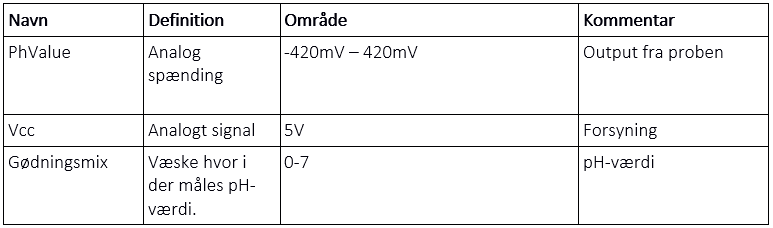
\includegraphics[scale=0.6]{../Projektdokumentation/Systemarkitektur/Graenseflader/Screenshots/tabel4_pH-probe.PNG}
	\caption{Grænsefladebeskrivelse: pH-probe}
	\label{screenshot:tabel4}
\end{figure}

\subsection{Jordfugt Grænsefladebeskrivelse}
Jordfugt måleren måler fugten i jorden. Her stikkes der nogle spyd ned i jorden, som giver en spænding ud afhængig af fugtigheden. PSoC'en omsætter denne spænding til en streng på I2C bussen.

\begin{figure}[H]
	\centering
	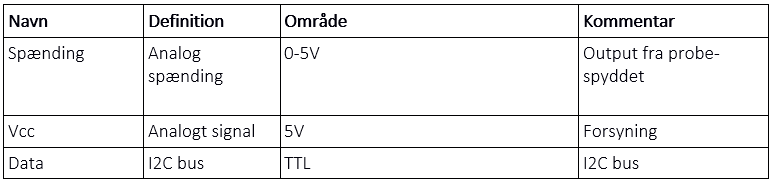
\includegraphics[scale=0.6]{../Projektdokumentation/Systemarkitektur/Graenseflader/Screenshots/tabel5_jordfugt.PNG}
	\caption{Grænsefladebeskrivelse: Jordfugt}
	\label{screenshot:tabel5}
\end{figure}



\newpage
\section{Kommunikations Protokol}
%!TEX root = ../../main.tex

\subsection{Overordnet}
Til kommunikation i AVS har vi valgt at implementere en protokol der bruges til kommunikation mellem hardware enheder.
Det drejer sig om to busser der følger samme format, samt er der gjort brug af I2C i forhold til følere. De to busser Kar og Ø bus basere sig begge på samme data format da deres fysiske lag er ens. Busserne kører master/slave kommunikation det gør at det kun er master der kan initiere kommunikation.\\\\

Til at kommunikere mellem GUI og CentralControl har vi designet endnu en protokol, som er uafhængig af ovenstående.

\subsection{Dataformat - Kar og Ø bus} 
Data bliver sendt på følgende format:

\begin{enumerate}
\item Adressen på modtager af besked
\item Adressen på afsender af besked
\item Længden af de kommende argumenter (kan være 0)
\item Kommando der ønskes behandlet
\item Argumenter i henhold til længden
\end{enumerate}

Systemet er inddelt i forespørgsler og svar, grundet master/slave formatet. Derfor kan en hel besked betragtes som en forespørgsel fra master og et svar fra slave.

Forespørgsler og svar har samme format som beskrevet ovenfor.

En kommunikation mellem master og slave kunne se således ud:
Master vil sende på dette format:
\begin{table}[H]
\setlength{\parindent}{12pt}
\begin{tabular}{|l|l|c|c|c|}\hline
\multicolumn{5}{|l|}{Master\cellcolor[gray]{0.9}}\\\hline
RxAddr & TxAddr & len & cmd & args \\\hline
1 Byte & 1 Byte & 1 Byte & 1 Byte & len * 1 Bytes \\\hline 
\end{tabular}
\end{table}


Slave vil svare på dette format:
\begin{table}[H]
\setlength{\parindent}{12pt}
\begin{tabular}{|l|l|c|c|c|}\hline
\multicolumn{5}{|l|}{Slave\cellcolor[gray]{0.7}}\\\hline
RxAddr & TxAddr & len & cmd & args  \\\hline
1 Byte & 1 Byte & 1 Byte & 1 Byte & len * 1 bytes \\\hline 
\end{tabular}
\end{table}

Alt efter hvilken kommando der sendes vil det variere om der er argumenter med det vil sige at len godt kan være 0. Som det også kan ses er master/slave forespørgsel og svar ens i opbygningen.

\subsection{Kar bus kommandoer}
Alle kommandoer er delt op på et "request" / "response" format dette er pga. af master/slave kommunikationen, det gør så at master altid kan forvente at få et svare og hvis ikke der bliver svaret er der sket en fejl.

Der er implementere følgende kommandoer på KarBus:

\begin{table}[H]
\setlength{\parindent}{12pt}
\begin{tabular}{|l|l|}\hline
\multicolumn{2}{|c|}{KarBus\cellcolor[gray]{0.7}}\\\hline
Kommando & Beskrivelse \\\hline
REQ\_KAR\_SENSOR\_DATA 		& Forespørgsel på at få data fra sensor der er koblet til kar \\\hline 
RES\_KAR\_SENSOR\_DATA 		& Svar indeholdende sensor data								 \\\hline 
REQ\_KAR\_VENTIL	   		& Forespørgsel på at skifte tilstand på ventil der er koblet til kar \\\hline 
RES\_KAR\_VENTIL       		& Svar der indeholder den tilstand ventilen er sat til \\\hline 
REQ\_KAR\_PUMPE		   		& Forespørgsel på at skifte hastighed på pumpen \\\hline 
RES\_KAR\_PUMPE 	   		& Svar indeholdende den hastighed pumpen der sat til \\\hline 
REQ\_KAR\_OPRET 	   		& Forespørgsel om at oprette en ny sensor ø \\\hline
RES\_KAR\_OPRET 	   		& Svar med adressen på den nye ø \\\hline 
REQ\_KAR\_OE\_LIST	   		& Forespørgsel om at oprette en ny sensor ø \\\hline
RES\_KAR\_OE\_LIST	   		& Svar med adressen på den nye ø \\\hline 
REQ\_KAR\_OE\_SENSOR\_DATA	& Forespørgsel på at få sensors øens sensor data \\\hline
RES\_KAR\_OE\_SENSOR\_DATA 	& Svar med data for sensor ø og om sensor er koblet til eller ej \\\hline 
REQ\_KAR\_OE\_VENTIL 	    & Forespørgsel om at åbne/lukke sensor øens ventil \\\hline
RES\_KAR\_OE\_VENTIL 	    & Svar med den tilstand ventilen er efterlad i \\\hline
REQ\_KAR\_OE\_SENSOR\_TYPE 	& Forespørgsel om hvilken type føler der er tilsluttet øen \\\hline
RES\_KAR\_OE\_SENSOR\_TYPE 	& Svar med sensor type \\\hline  
\end{tabular}
\end{table}

\subsubsection{REQ\_KAR\_SENSOR\_DATA}
Denne kommando er en forespørgsel på data som Karrets sensorer har indsamlet.

\begin{table}[H]
\setlength{\parindent}{12pt}
\begin{tabular}{|l|lcc|}
\hline
\multicolumn{4}{|c|}{Kommado med argumenter}\\\hline
Kommando & 0x1 & & \\
Argumenter & ingen & & \\\hline
\end{tabular}
\end{table}



\subsubsection{RES\_KAR\_SENSOR\_DATA}
Denne kommando er et svar der indeholder den data karrets sensorer har indsamlet.

\begin{table}[H]
\setlength{\parindent}{12pt}
\begin{tabular}{|l|lcc|}
\hline
\multicolumn{4}{|c|}{Kommado med argumenter}\\\hline
Kommando & 0x2 & & \\
Argumenter & ID & Value1 & Value2 \\\hline
\end{tabular}
\end{table}

Argumenterne kan forekomme flere gange og vil være reflekteret i længden. Det vil sige at en længde på 3 i dette tilfælde betyder at der kun er indeholdt en sensor i svaret, hvis længden var 6 ville der være to sensorer osv.

\begin{table}[H]
\setlength{\parindent}{12pt}
\begin{tabular}{|l|l|}
\hline
\multicolumn{2}{|c|}{Argument uddybning}\\\hline
ID & Dette er følerens identifikation alt efter om det er pH, flow eller andet der bliver målt. \\
Value1 & Er heltals værdien af den målte størrelse. \\
Value2 & Hvis MSB'en i denne er sat betyder det at der skal lægges en halv til value1.\\\hline
\end{tabular}
\end{table}


\subsubsection{REQ\_KAR\_VENTIL}
Denne kommando er en forespørgsel på at styre karrets ventiler.

\begin{table}[H]
\setlength{\parindent}{12pt}
\begin{tabular}{|l|lcc|}
\hline
\multicolumn{4}{|c|}{Kommado med argumenter}\\\hline
Kommando & 0x3 & & \\
Argumenter & ID & STATE & \\\hline
\end{tabular}
\end{table}

Her er ID den ventil der ønske manipuleret og STATE er hvilken tilstand der ønskes at ventilen skal stå i.\\\\
STATE kan være følgende:
\begin{table}[H]
\setlength{\parindent}{12pt}
\begin{tabular}{|l|l|}
\hline
\multicolumn{2}{|c|}{Argumenter uddybet}\\\hline
Lukket & 0x0 \\
Åben & 0x1 \\\hline
\end{tabular}
\end{table}

\subsubsection{RES\_KAR\_VENTIL}
Denne kommando er et svar der indeholder den tilstand ventilen er i.

\begin{table}[H]
\setlength{\parindent}{12pt}
\begin{tabular}{|l|lcc|}
\hline
\multicolumn{4}{|c|}{Kommado med argumenter}\\\hline
Kommando & 0x4 & & \\
Argumenter & STATE & & \\\hline
\end{tabular}
\end{table}

Svaret på en ventil forespørgsel er hvilken tilstand ventilen er blevet sat til.

\subsubsection{REQ\_KAR\_PUMPE}
Denne kommando er en forespørgsel på at styre karrets pumpe.

\begin{table}[H]
\setlength{\parindent}{12pt}
\begin{tabular}{|l|lcc|}
\hline
\multicolumn{4}{|c|}{Kommado med argumenter}\\\hline
Kommando & 0x5 & & \\
Argumenter & STATE & & \\\hline
\end{tabular}
\end{table}

Da pumpen kan køre med flere hastigheder sendes der en state der kan være følgende:

\begin{table}[H]
\setlength{\parindent}{12pt}
\begin{tabular}{|l|l|}
\hline
\multicolumn{2}{|c|}{Argumenter uddybet}\\\hline
Slukket & 0 \\
Lav hastighed & 25 \\
Middel hastighed & 50 \\
Høj hastighed & 75 \\\hline
\end{tabular}
\end{table}

Tallene betyder hvor mange procent duty cycle PWM signalet der styrer pumpen skal sættes til dvs, 50 er en duty cycle på 50\%.

\subsubsection{RES\_KAR\_PUMPE}
Denne kommando er et svar der indeholder den tilstand pumpen er i.

\begin{table}[H]
\setlength{\parindent}{12pt}
\begin{tabular}{|l|lcc|}
\hline
\multicolumn{4}{|c|}{Kommado med argumenter}\\\hline
Kommando & 0x6 & & \\
Argumenter & STATE & & \\\hline
\end{tabular}
\end{table}


Svaret på en pumpe forespørgsel er hvilken tilstand pumpen er blevet sat til. Altså om den er slukket eller kører med en af de tre hastigheder.


\subsubsection{REQ\_KAR\_OPRET}
Denne kommando er en forespørgsel give en sensorø der er koblet på et kar en adresse.

\begin{table}[H]
\setlength{\parindent}{12pt}
\begin{tabular}{|l|lcc|}
\hline
\multicolumn{4}{|c|}{Kommado med argumenter}\\\hline
Kommando & 0x7 & & \\
Argumenter & ADDR & & \\\hline
\end{tabular}
\end{table}


\subsubsection{RES\_KAR\_OPRET}
Denne kommando er et svar der fortæller om det lykkedes at oprette sensorøen på karret.

\begin{table}[H]
\setlength{\parindent}{12pt}
\begin{tabular}{|l|lcc|}
\hline
\multicolumn{4}{|c|}{Kommado med argumenter}\\\hline
Kommando & 0x8 & & \\
Argumenter & ADDR & & \\\hline
\end{tabular}
\end{table}


\subsubsection{REQ\_KAR\_OE\_LIST}
Denne kommando er en forespørgsel på at få af vide hvilke ø'er der er oprettede .

\begin{table}[H]
\setlength{\parindent}{12pt}
\begin{tabular}{|l|lcc|}
\hline
\multicolumn{4}{|c|}{Kommado med argumenter}\\\hline
Kommando & 0x9 & & \\
Argumenter & ingen & & \\\hline
\end{tabular}
\end{table}


\subsubsection{RES\_KAR\_OE\_LIST}
Denne kommando er et svar der fortæller hvilke ø'er der er koblet til karret. Der returneres 1 adresse per ø.

\begin{table}[H]
\setlength{\parindent}{12pt}
\begin{tabular}{|l|lcc|}
\hline
\multicolumn{4}{|c|}{Kommado med argumenter}\\\hline
Kommando & 0xA & & \\
Argumenter & ADDR & & \\\hline
\end{tabular}
\end{table}

\subsubsection{REQ\_KAR\_OE\_SENSOR\_DATA}
Denne kommando er en forespørgsel at få data fra de sensorer der er tilkoblet en sensorø. Argumentet er adressen på den ø der ønskes at der skal læses fra.

\begin{table}[H]
\setlength{\parindent}{12pt}
\begin{tabular}{|l|lcc|}
\hline
\multicolumn{4}{|c|}{Kommado med argumenter}\\\hline
Kommando & 0xB & & \\
Argumenter & ADDR & & \\\hline
\end{tabular}
\end{table}


\subsubsection{RES\_KAR\_OE\_SENSOR\_DATA}
Denne kommando er et svar der indeholder den data sensorø'en har opsamlet.

\begin{table}[H]
\setlength{\parindent}{12pt}
\begin{tabular}{|l|lccc|}
\hline
\multicolumn{5}{|c|}{Kommado med argumenter}\\\hline
Kommando & 0xC & & & \\
Argumenter & FS\_ADDR & FS\_STATUS & VALUE1 & VALUE2 \\\hline
\end{tabular}
\end{table}

Argumenterne beskrives her:

\begin{table}[H]
\setlength{\parindent}{12pt}
\begin{tabular}{|l|l|}
\hline
\multicolumn{2}{|c|}{Argumenter uddybet}\\\hline
FS\_ADDR 	& Dette er adressen på selve fieldsensoren \\
FS\_STATUS	& Status indikere om fieldsensoren er online (1) eller offline (0) \\
VALUE1 		& Heltals værdien af det sensoren udlæser \\
VALUE2 		& Hvis MSB er sat i denne indikere den at der er en halv der skal lægge til heltals værdien \\\hline
\end{tabular}
\end{table}

\subsubsection{REQ\_KAR\_OE\_VENTIL}
Denne kommando er en forespørgsel at åbne en ø ventil.

\begin{table}[H]
\setlength{\parindent}{12pt}
\begin{tabular}{|l|lcc|}
\hline
\multicolumn{4}{|c|}{Kommado med argumenter}\\\hline
Kommando & 0xD & & \\
Argumenter & OE\_ADDR & STATE & \\\hline
\end{tabular}
\end{table}

State er om ventilen skal være åben(1) eller lukket(0).

\subsubsection{RES\_KAR\_OE\_VENTIL}
Denne kommando er et svar der fortæller om det lykkedes at åbne ventilen det gøres ved at returnere den tilstand ventilen er i state har samme betydning som ovenfor.

\begin{table}[H]
\setlength{\parindent}{12pt}
\begin{tabular}{|l|lcc|}
\hline
\multicolumn{4}{|c|}{Kommado med argumenter}\\\hline
Kommando & 0xE & & \\
Argumenter & STATE & & \\\hline
\end{tabular}
\end{table}

State er om ventilen er åben(1) eller lukket(0).

\subsubsection{REQ\_KAR\_OE\_SENSOR\_TYPE}
Denne kommando er en forespørgsel på at få afvide hvilken type sensor der er koblet til en bestemt fieldsensor adresse.

\begin{table}[H]
\setlength{\parindent}{12pt}
\begin{tabular}{|l|lcc|}
\hline
\multicolumn{4}{|c|}{Kommado med argumenter}\\\hline
Kommando & 0xF & & \\
Argumenter & OE\_ADDR & FS\_ADDR & \\\hline
\end{tabular}
\end{table}


\subsubsection{RES\_KAR\_OE\_SENSOR\_TYPE}
Denne kommando er et svar der indeholder typen på den sensor der blev spurgt på.

\begin{table}[H]
\setlength{\parindent}{12pt}
\begin{tabular}{|l|lcc|}
\hline
\multicolumn{4}{|c|}{Kommado med argumenter}\\\hline
Kommando & 0x10 & & \\
Argumenter & TYPE & & \\\hline
\end{tabular}
\end{table}

Type kan være ??.

\subsection{Ø bus kommandoer}
Alle kommandoer er delt op på et "request" / "response" format dette er pga. af master/slave kommunikationen, det gør så at master altid kan forvente at få et svare og hvis ikke der bliver svaret er der sket en fejl.

Der er implementere følgende kommandoer på ØBussen:

\begin{table}[H]
\setlength{\parindent}{12pt}
\begin{tabular}{|l|l|}\hline
\multicolumn{2}{|c|}{ØBus\cellcolor[gray]{0.7}}\\\hline
Kommando & Beskrivelse \\\hline
REQ\_OE\_FS\_DATA 		& Forespørgsel på at få data fra sensor der er koblet til Sensor Ø \\\hline 
REQ\_OE\_FS\_DATA 		& Svar indeholdende sensor data								 \\\hline 
REQ\_OE\_VENTIL	   		& Forespørgsel på at skifte tilstand på ventil der er koblet til Sensor Ø \\\hline 
REQ\_OE\_VENTIL       		& Svar der indeholder den tilstand ventilen er sat til \\\hline 
\end{tabular}
\end{table}

\subsubsection{REQ\_OE\_FS\_DATA}
Denne kommando er en forespørgsel på data som Sensor Øen sensorer har indsamlet.

\begin{table}[H]
\setlength{\parindent}{12pt}
\begin{tabular}{|l|lcc|}
\hline
\multicolumn{4}{|c|}{Kommado med argumenter}\\\hline
Kommando & 0x1 & & \\
Argumenter & ingen & & \\\hline
\end{tabular}
\end{table}



\subsubsection{RES\_OE\_FS\_DATA}
Denne kommando er et svar der indeholder den data karrets sensorer har indsamlet.

\begin{table}[H]
\setlength{\parindent}{12pt}
\begin{tabular}{|l|lcccc|}
\hline
\multicolumn{6}{|c|}{Kommado med argumenter}\\\hline
Kommando & 0x2 & & & & \\
Argumenter & Addr & Type & Status & Value1 & Value2 \\\hline
\end{tabular}
\end{table}

Argumenterne gentages per Fieldsensor der er tilkoblet

\begin{table}[H]
\setlength{\parindent}{12pt}
\begin{tabular}{|l|l|}
\hline
\multicolumn{2}{|c|}{Argument uddybning}\\\hline
Addr & Adresse på Fieldsensoren. \\
Type & Type af Fieldsensoren. \\
Status & Status på Fieldsensoren 0x01 er aktiv og 0x00 svarer ikke. \\
Value1 & Er heltals værdien af den målte størrelse. \\
Value2 & Hvis MSB'en i denne er sat betyder det at der skal lægges en halv til value1.\\\hline
\end{tabular}
\end{table}

\subsubsection{REQ\_OE\_VENTIL}
Denne kommando er en forespørgsel på at styre Sensor Ø'ens ventiler.

\begin{table}[H]
\setlength{\parindent}{12pt}
\begin{tabular}{|l|lcc|}
\hline
\multicolumn{4}{|c|}{Kommado med argumenter}\\\hline
Kommando & 0x3 & & \\
Argumenter & ID & STATE & \\\hline
\end{tabular}
\end{table}

Her er ID den ventil der ønske manipuleret og STATE er hvilken tilstand der ønskes at ventilen skal stå i.\\\\
STATE kan være følgende:
\begin{table}[H]
\setlength{\parindent}{12pt}
\begin{tabular}{|l|l|}
\hline
\multicolumn{2}{|c|}{Argumenter uddybet}\\\hline
Lukket & 0x0 \\
Åben & 0x1 \\\hline
\end{tabular}
\end{table}

\subsubsection{RES\_OE\_VENTIL}
Denne kommando er et svar der indeholder den tilstand ventilen er i.

\begin{table}[H]
\setlength{\parindent}{12pt}
\begin{tabular}{|l|lcc|}
\hline
\multicolumn{4}{|c|}{Kommado med argumenter}\\\hline
Kommando & 0x4 & & \\
Argumenter & STATE & & \\\hline
\end{tabular}
\end{table}

Svaret på en ventil forespørgsel er hvilken tilstand ventilen er blevet sat til.


\subsection{GUI Protokol}

Til at kommunikere mellem GUI og CentralControl benyttes en TCP/IP forbindelse. Herunder er protokollen beskrevet.\\\\

